\section{Introduction}
In this chapter are reported the evaluation performed for the Kundera extensions.
To support the implementation of the Kundera extensions, as described in chapter \ref{chap:kundera}, we have adopted a test driven approach; in section \ref{sec:crud}, those tests are described in detail.
\noindent We will provide, in section \ref{sec:performance}, a comparison of the performance of the developed Kundera extensions in terms of throughput and latency. To measure those metrics we have used Yahoo Cloud Serving Benchmark (YCSB) \cite{paper:ycsb} since it was already used by the Kundera team to test the other implemented Kundera clients and since we wanted to compare our results to their.

\section{Test CRUD operations}
\label{sec:crud}
The Kundera extensions development, due to the lack of information both in the documentation and from the community, has been approached in a test driven way.
The first step was to write the required JUnit tests, one for each feature we have planned to support.

\newparagraph We primarily wanted to achieve code portability of the application model classes, this should be exploited by the usage of the JPA interface but, as stated in chapter \ref{chap:ps}, there were problems in the old NoSQL service implementation relatively to this point.
Secondary we want to be sure that, while entities are persisted in the underlying NoSQL database, they can be restored without any loss of information and thus, the mapping between entities and the NoSQL database data model, behaves correctly in both verses.
Hence, the extensions cannot be tested directly by testing single methods behavior of the extensions classes, this will for sure test the correctness of the operations but, since Kundera clients are not obliged to follow a rigid structure for their code in the implementation of the required interfaces, tests written for a client are not guaranteed to run correctly for another one. 

\noindent The approach we adopted was to define a single test suite, that will test each  of the features we planned to support, by interacting directly with Kundera through the JPA interface. This makes us able to use the same tests independently of the specific extension and, thus, testing the correctness of CRUD operations through the JPA interface and the portability of the code by means of tests portability.

\noindent Those tests have been primarily used to test the extensions during the development against the local emulator of both Google Datastore and Azure Tables, but they have also been executed on the remote database instances by connecting to them through the network from the development machine. This tests have been made to guarantee the correct functioning of the two extensions on the real database instances, since tests executed locally, are executed against emulators of real systems.

\subsection{Tests structure}
Tests are composed by the entities to be persisted, annotated with the JPA annotations, and a test class for each feature.
There are 20 defined entities that include:
\begin{itemize}
\item simple entities related with the JPA relationships annotations, used to test relationships among entities;
\item embeddable entities and specific entities that use those embeddable entities as data types, both used to test the embedded feature of the JPA;
\item entities with enum fields, used to test the enum fields support;
\item entities declared with different data types for the primary key identifier, used to test ids auto-generation and user-defined ids validation.
\end{itemize}

\noindent The test classes, developed for testing the correctness of relationships, are:
\begin{itemize}
\item \texttt{MTMTest}, to test the \textit{Many to Many} relationship type;
\item \texttt{MTOTest}, to test the \textit{Many to One} relationship type;
\item \texttt{OTMTest}, to test the \textit{One to Many} relationship type;
\item \texttt{OTOTest}, to test the \textit{One to One} relationship type;
\end{itemize}
\noindent All of those test classes implement two different methods: \texttt{testCRUD()}, that test the relationship by interacting with the method of the \texttt{EntityManager} interface, and \texttt{testQuery()}, that tests the relationships by reading, updating and deleting entities through JPQL queries.

\newparagraph The remaining tests classes are:
\begin{itemize}
\item \texttt{ElementCollectionTest}, that tests the JPA feature of persisting list of objects as entity fields;
\item \texttt{EmbeddedTest}, that tests the JPA feature of persisting user-defined as entity fields;
\item \texttt{EnumeratedTest}, that tests the Jsupport for enum fields;
\item \texttt{QueryTest}, that tests the execution of \textit{SELECT} queries and the support for the various JPQL clauses in queries.
\end{itemize}

\newparagraph In figure \ref{fig:test-uml} is reported the class diagram of the various test classes.

\begin{figure}[tbh]
  \centering
  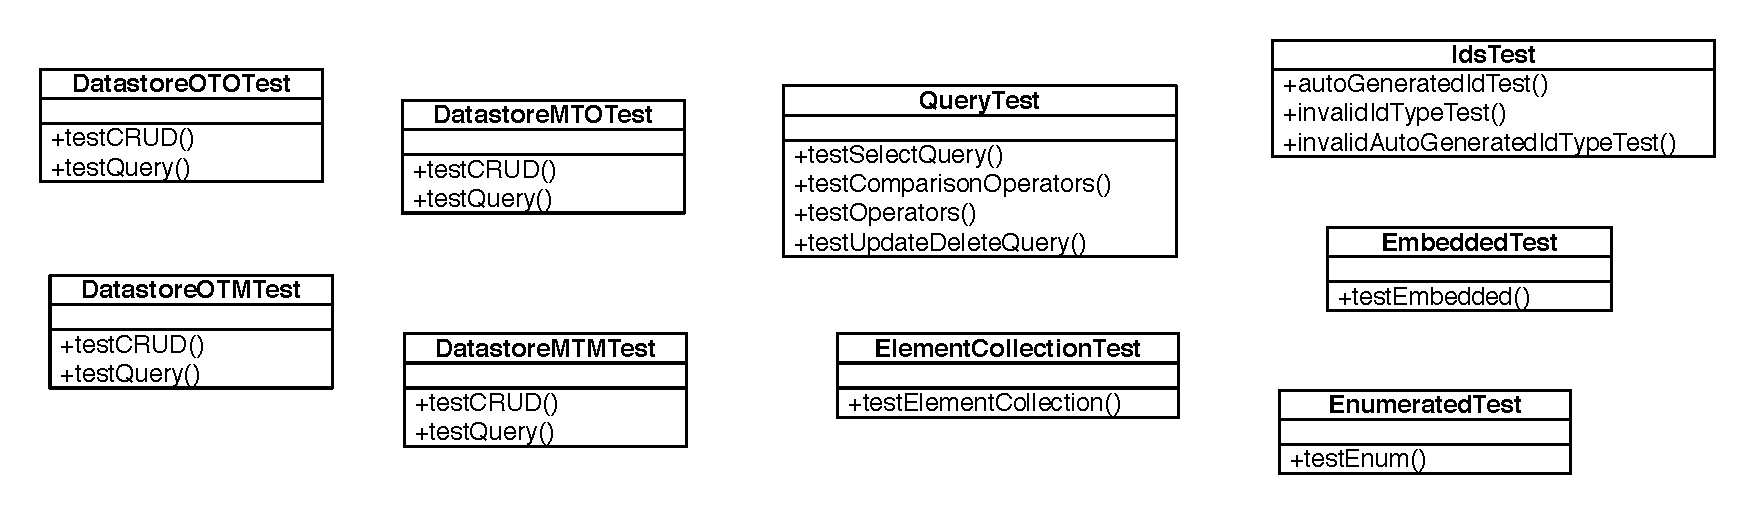
\includegraphics[width=14cm]{images/test_uml}
  \caption{Class diagram of the test classes}
  \label{fig:test-uml}
\end{figure} 

\section{Performance tests}
\label{sec:performance}
We wanted to test the overhead of the developed Kundera extensions with respect to direct use of low-level APIs. To test those kind of performance in terms of throughput and latency of the read and write operations, we have used Yahoo Cloud Serving Benchmark.
We choose this approach since it was already used by Kundera developers to estimate the overhead that Kundera adds to the low-level API versions of its clients. In this way, it is possible to compare our extensions with those developed by other Kundera contributors.

\subsection{Yahoo Cloud Serving Benchmark}
Yahoo Cloud Serving Benchmark (YCSB) is a framework with the general goal of facilitating performance comparisons of the new generations of cloud serving systems \cite{paper:ycsb}.

\noindent YCSB provides the facility to benchmark various NoSQL database systems such Apache Cassandra, DynamoDB, Voldemort, MongoDB and many others.
The key feature of the benchmark system is extensibility, it in facts supports easy definition of new \textit{workloads} and new systems to benchmark.

\begin{figure}[tbh]
  \centering
  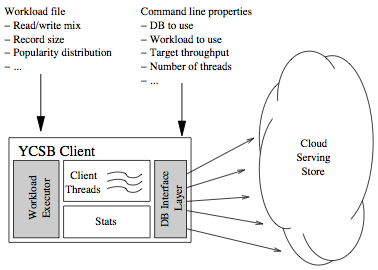
\includegraphics[width=10cm]{images/ycsb_architecture}
  \caption{YCSB architecture \cite{paper:ycsb}}
  \label{fig:ycsb-architecture}
\end{figure} 

\newparagraph The access point to the benchmark framework is the \textit{YCSB Client} which is responsible of generating the operations which make up the workload; the workload is then executed by the \textit{Workload executor} that drives multiple client threads, which in turn execute a sequential series of operations by making calls to the \textit{database interface layer}.

\noindent The workloads are executed in two separate phases:
\begin{enumerate}
\item the \textbf{load phase}, which loads the workload data to the database system;
\item the \textbf{transaction phase}, which executes the workload on the loaded data.
\end{enumerate}
\noindent Each thread rules the rate at which it generates requests and measures the latency and the throughput of its operations. At the end of the benchmark, the statistics module aggregates the measurements and builds a report.

\subsection{YCSB adapters}
The YCSB Client abstracts from the specific database system under test through the \textit{database interface layer}; this allows YCSB to generate operations like ``read record'' or ``update record'', without having to understand the specific API of the underlying database.

\noindent To create a database adapter, the abstract class \texttt{com.yahoo.ycsb.DB} must be extended and the following methods need to be implemented:
\begin{itemize}
\item \texttt{init()}, which is used to perform any initialization operation such as connecting to the database instance and it is called once per thread;
\item \texttt{read(String table, String key, ...)}, which is supposed to read the given record;
\item \texttt{scan(String table, String startkey, int recordcount, ...)}, which is supposed to perform a range scan;
\item \texttt{insert(String table, String key, ...)}, which is supposed to insert the given record;
\item \texttt{delete(String table, String key)}, which is supposed to delete the given record.
\end{itemize}

\newparagraph We developed  several YCSB adapters:
\begin{itemize}
\item an adapter for Google Datastore low-level API
\item an adapter for Google Datastore through the developed Kundera extension
\item an adapter for Azure Tables low-level API
\item an adapter for Azure Tables through the developed Kundera extension
\end{itemize}
\noindent Furthermore we have re-written the adapters for HBase both the Kundera version and the low-level API version. This has been necessary since the YCSB adapter for HBase, written by the Kundera team, were outdated and was not working anymore with the latest versions of HBase.

\subsubsection{Kundera adapters}
Regarding the Kundera version of the adapters, the same structure has been kept for all three databases. The \texttt{EntityManagerFactory} is instantiated at construction time since this operation causes Kundera to initialize all its internal structure; an instance of the entity manager is created in the \texttt{init} method since, the initialization of the \texttt{EntityManager} causes the initialization of the specific Kundera client; in this way each thread will have its own instance of the \texttt{EntityManager} with which interacting.
Apart from the \texttt{scan} method, which was not implemented since this operation is never issued during the workload we want to execute, every other operations calls the responsible method on the \texttt{EntityManager}, in the code \ref{code:insert-operation} is shown an example for the insert operation.

\begin{lstlisting}[language=Java, caption=Insert operation of the Azure Tables adapter, label=code:insert-operation]
@Override
public int insert(String table, String key, ...) {
    ...
    try {
        AzureTableUser user = new AzureTableUser(key, nextString(),, ...);
        em.persist(user);
        if (timeToClearEntityManager()) {
            em.clear();
        }
        return OK;
    } catch (Exception e) {
        return ERROR;
    }
}
\end{lstlisting}

\noindent In the code \ref{code:insert-operation} there are two elements that need a deep explanation. The first thing to notice is that an instance of \texttt{AzureTableUser} is persisted, in fact, we were not able to persist the entities generated by YCSB because, to be able to persist an entity with the JPA, we need an annotated class which should be then listed in the \textit{persistence.xml} file. For this reasons three different user class and three different persistence units have been defined:
\begin{itemize}
\item \texttt{AzureTableUser}, which refers to \texttt{kundera\textunderscore azure\textunderscore pu}, the persistence unit with the configuration for Azure Tables;
\item \texttt{DatastoreUser}, which refers to \texttt{kundera\textunderscore datastore\textunderscore pu}, the persistence unit with the configuration for Google Datastore;
\item \texttt{HBaseUser}, which refers to \texttt{kundera\textunderscore hbase\textunderscore pu}, the persistence unit with the configuration for Hbase.
\end{itemize} 
\noindent The second thing to notice is the call to the \texttt{timeToClearEntityManager()} method, which returns \texttt{true} each time 500 entities are persisted, this causes a clear of the persistence cache by calling \texttt{EntityManager.clear()}. If this operation is not performed, entities read can occur within the persistence cache bypassing the request to the underling database. We choose to clear the cache every 500 entities, in our workloads of 100.000 entities, to maintain the same proportion with the one used by Kundera in their test, in which the persistence cache is cleared every 5.000 entities on workloads of 1 million operations.

\subsubsection{Low-level API adapters}
Also the adapters for the low-level API version follows the same general structure. The connection to the database is performed, through low-level API, in the \texttt{init} method, to have a common behavior with respect to the Kundera adapters. Read, insert and delete operations are performed by a call to the specific low-level API, while the \texttt{scan} method has not been implemented.

\noindent The \texttt{init} method uses the properties defined in the property files specified in the execution command of the benchmark, to locate the remote database and instantiate a connection.

\subsection{YCSB tests}
YCSB comes with a core set of workloads, each workload represents a particular mix of read and write operations and defines the total number of operations that should be executed. 
\noindent YCSB benchmarks are executed in two separate phases and each of them generates a report. From the report of the \textit{load} phase, since this phase is responsible of storing the data required to run the workload to the target database, we obtain information about the throughput and the latency for the write operation. From the \textit{transaction} phase we want to obtain information about throughput and latency for the read operation. To do so, we run a custom workload composed of 100.000 operations entirely of type read so that the \textit{transaction} phase will generate the statistics we need.
\noindent Defined the adapters and the workload we were able to execute the tests.

\subsubsection{Google Datastore tests}
The tests for Google Datastore have been executed over a remote Datastore instance in a billed application billed and configured to accept remote API execution.

\noindent The results of the tests for the read operation are reported in figure \ref{fig:gae-test-read} whereas figure \ref{fig:gae-test-write} reports the results for the write operation.
 
\begin{figure}[tbh]
  \centering
  \subfloat[Throughput]{
    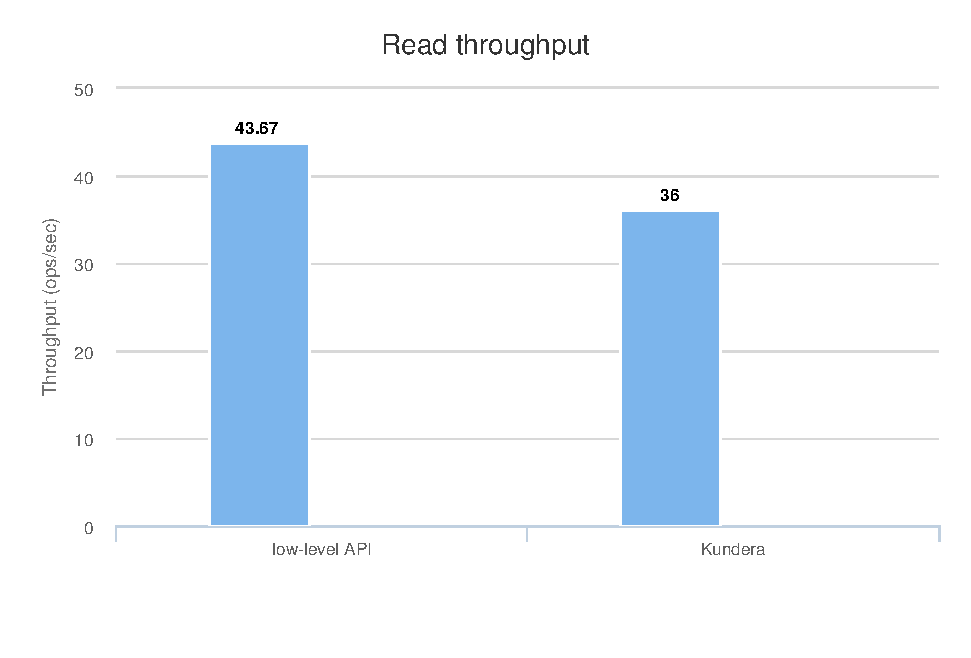
\includegraphics[width=7cm]{images/gae_read_throughput}
  }
  \subfloat[Latency]{
    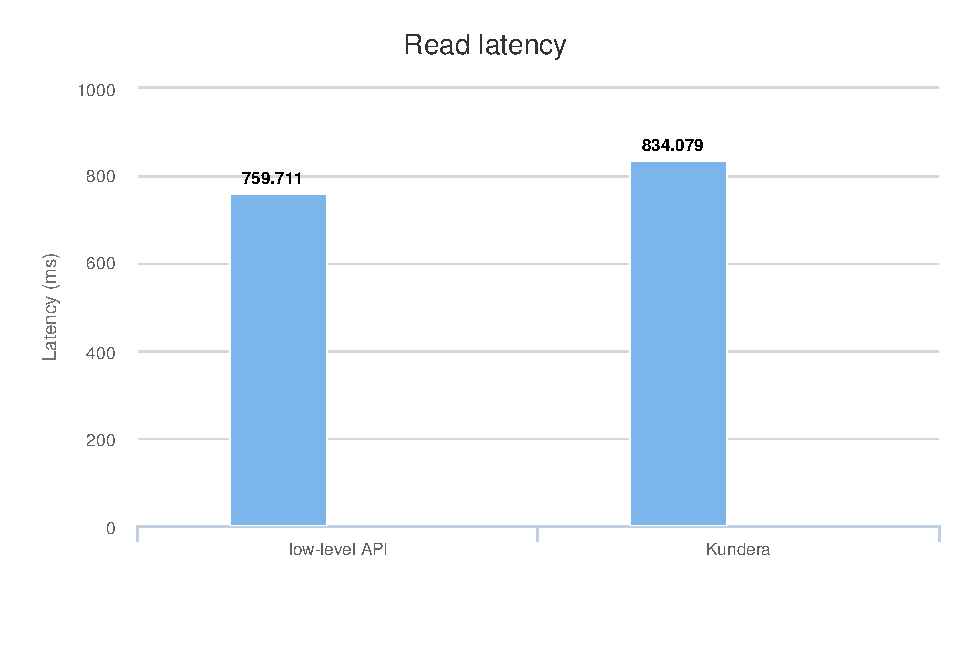
\includegraphics[width=7cm]{images/gae_read_latency}
  }
  \caption{Google Datastore - read operation benchmark results}
  \label{fig:gae-test-read}
\end{figure} 

\begin{figure}[tbh]
  \centering
  \subfloat[Throughput]{
    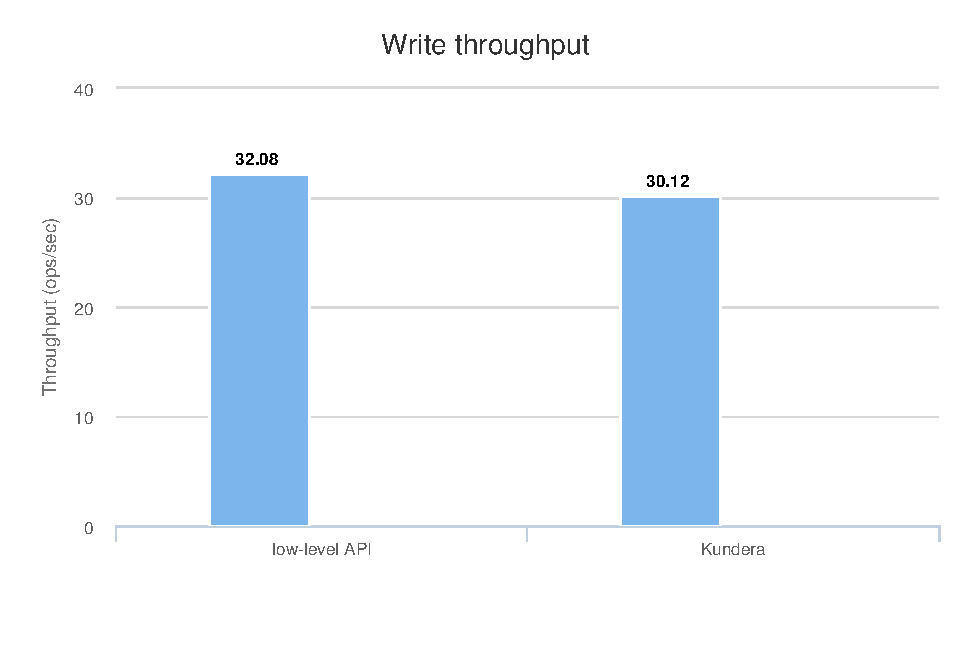
\includegraphics[width=7cm]{images/gae_write_throughput}
  }
  \subfloat[Latency]{
    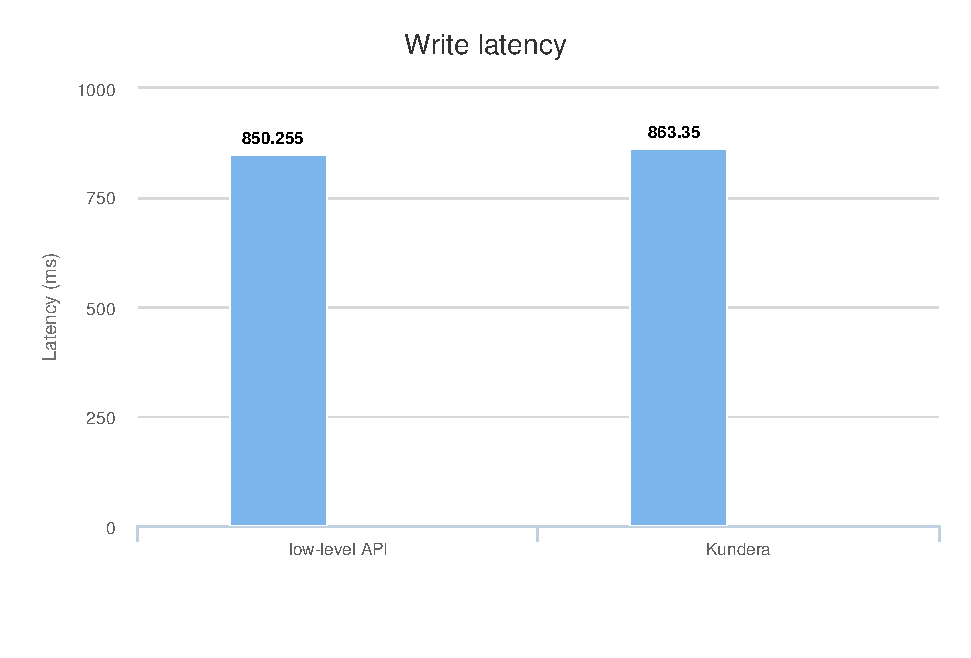
\includegraphics[width=7cm]{images/gae_write_latency}
  }
  \caption{Google Datastore - write operation benchmark results}
  \label{fig:gae-test-write}
\end{figure} 
 
\noindent The throughput of the Kundera version of the adapter shows in both cases a lower value compared to the result of low level API; as regards latency, the operations performed by the Kundera version of the adapter shows a higher latency with respect to the low API version. However the overhead introduced by Kundera and the Google Datastore extension, measured in terms of latency and throughput, is very low compared to use of the low-level API, both for the read and for the write operation.

\subsubsection{Azure Tables tests}
The tests for Azure Tables have been executed over a remote storage instance deployed in Azure.

\noindent The results of the tests for the read operation are reported in figure \ref{fig:azure-test-read} whereas figure \ref{fig:azure-test-write} reports the results for the write operation.
 
\begin{figure}[tbh]
  \centering
  \subfloat[Throughput]{
    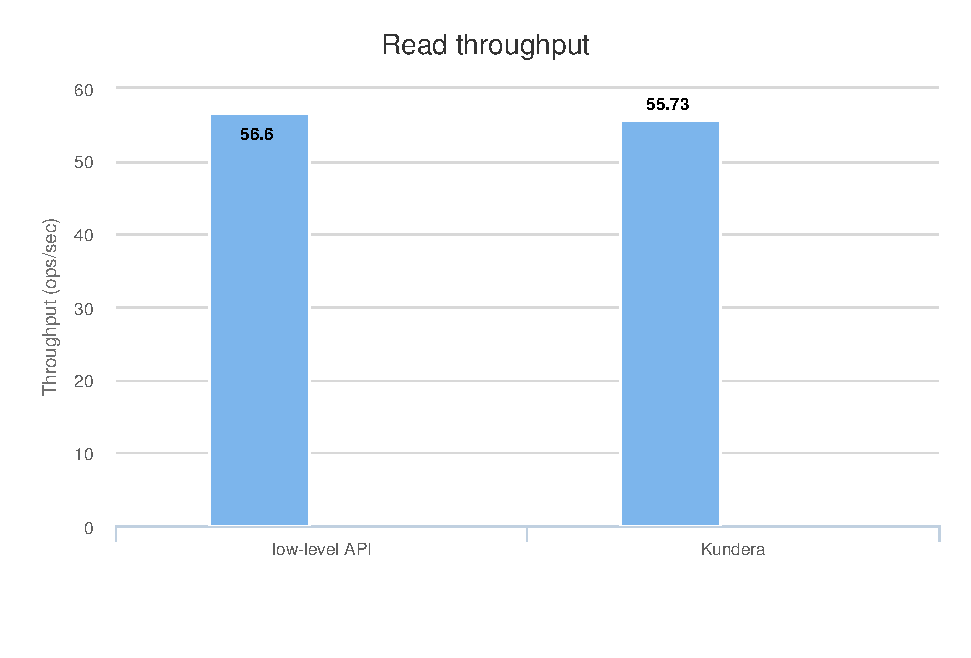
\includegraphics[width=7cm]{images/azure_read_throughput}
  }
  \subfloat[Latency]{
    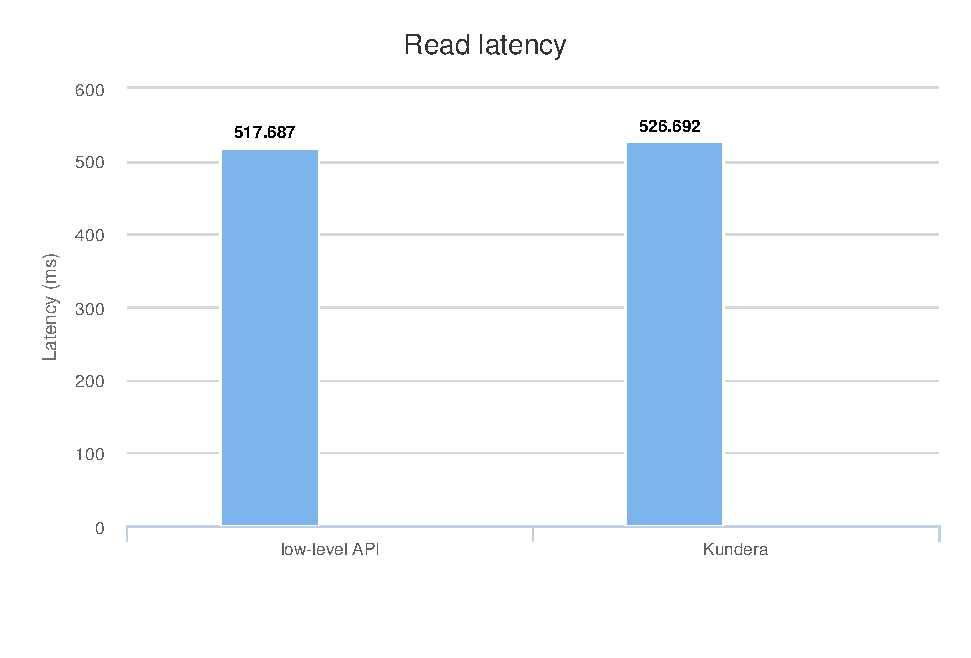
\includegraphics[width=7cm]{images/azure_read_latency}
  }
  \caption{Azure Tables - read operation benchmark results}
  \label{fig:azure-test-read}
\end{figure} 

\begin{figure}[tbh]
  \centering
  \subfloat[Throughput]{
    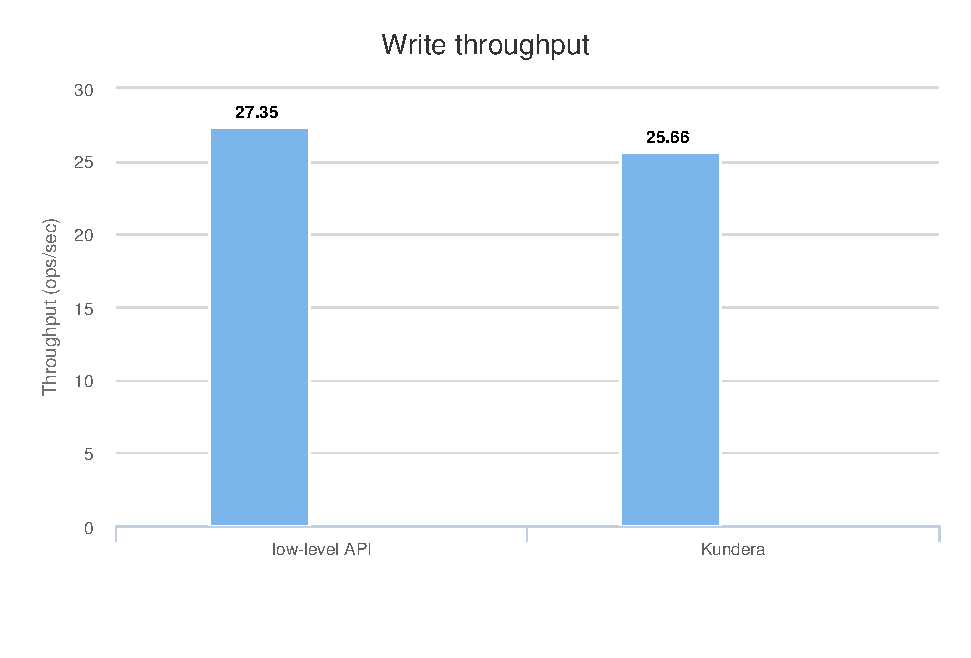
\includegraphics[width=7cm]{images/azure_write_throughput}
  }
  \subfloat[Latency]{
    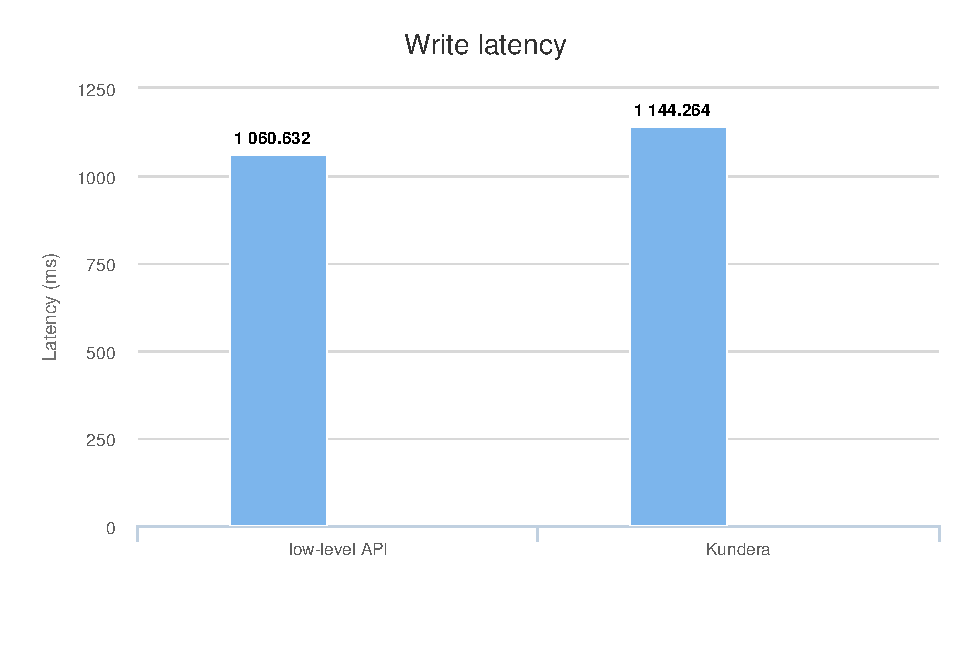
\includegraphics[width=7cm]{images/azure_write_latency}
  }
  \caption{Azure Tables - write operation benchmark results}
  \label{fig:azure-test-write}
\end{figure} 

\noindent Also for Azure Tables, as for Google Datastore, we have observed a throughput loss of the Kundera adapter with respect to the low level API version and the higher latency. The loss in performance in this case is not as much as in Google Datastore and thus also here we can conclude that the overhead introduced by Kundera and the Azure Tables extension, measured in terms of latency and throughput, is very low compared to use of the low-level API, both for the read and for the write operation.

\subsubsection{HBase tests}
HBase test should have been executed over an instance of HBase, in full distributed configuration, in the cloud of Politecnico di Milano but due to a failure of the host machines the tests could not be performed.

\noindent In figure \ref{fig:hbase-test-read} and \ref{fig:hbase-test-write} are reported the results obtained while testing the HBase adapters. They have been executed on a workload of 1.000 entities in a locally installed instance of HBase.

\begin{figure}[tbh]
  \centering
  \subfloat[Throughput]{
    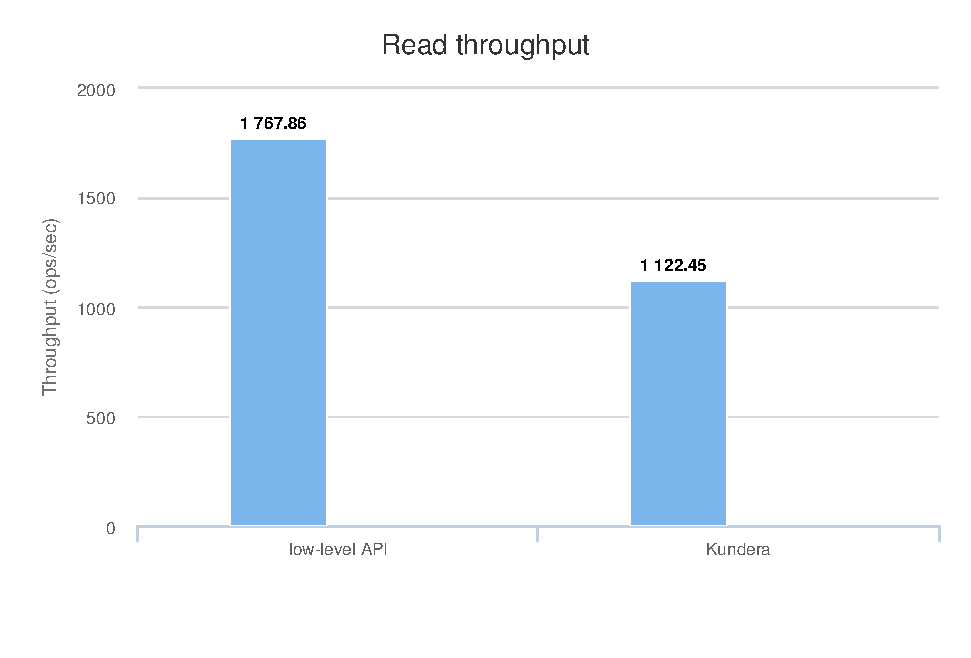
\includegraphics[width=7cm]{images/hbase_read_throughput}
  }
  \subfloat[Latency]{
    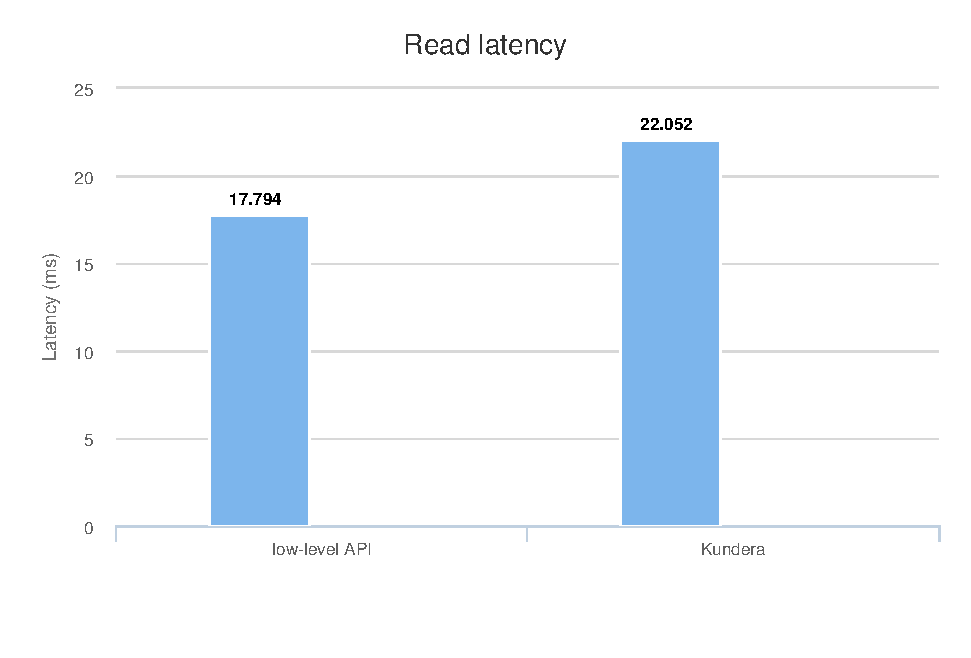
\includegraphics[width=7cm]{images/hbase_read_latency}
  }
  \caption{HBase - read operation benchmark results}
  \label{fig:hbase-test-read}
\end{figure} 

\begin{figure}[tbh]
  \centering
  \subfloat[Throughput]{
    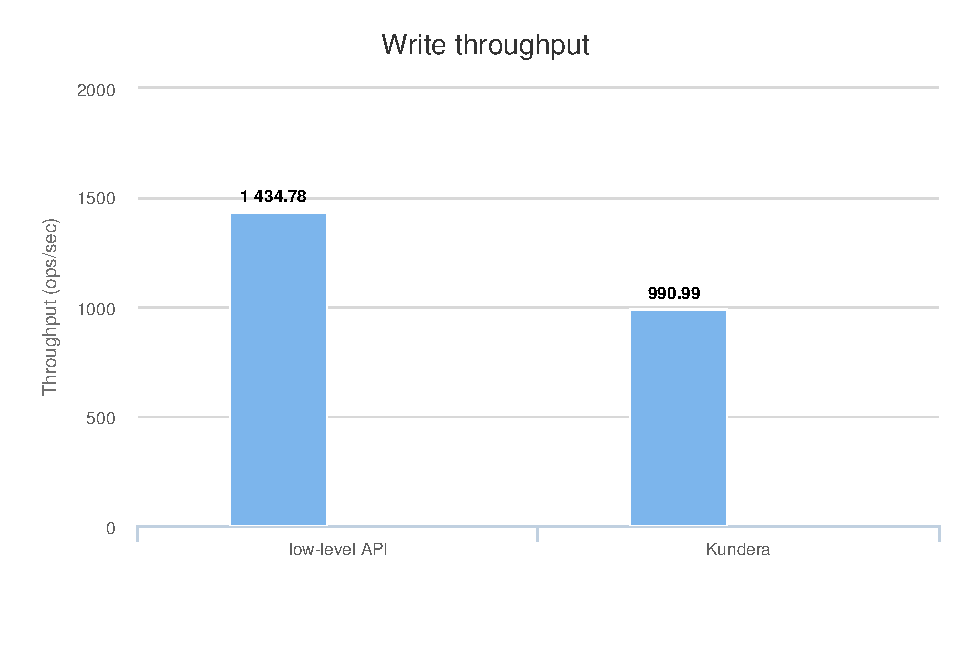
\includegraphics[width=7cm]{images/hbase_write_throughput}
  }
  \subfloat[Latency]{
    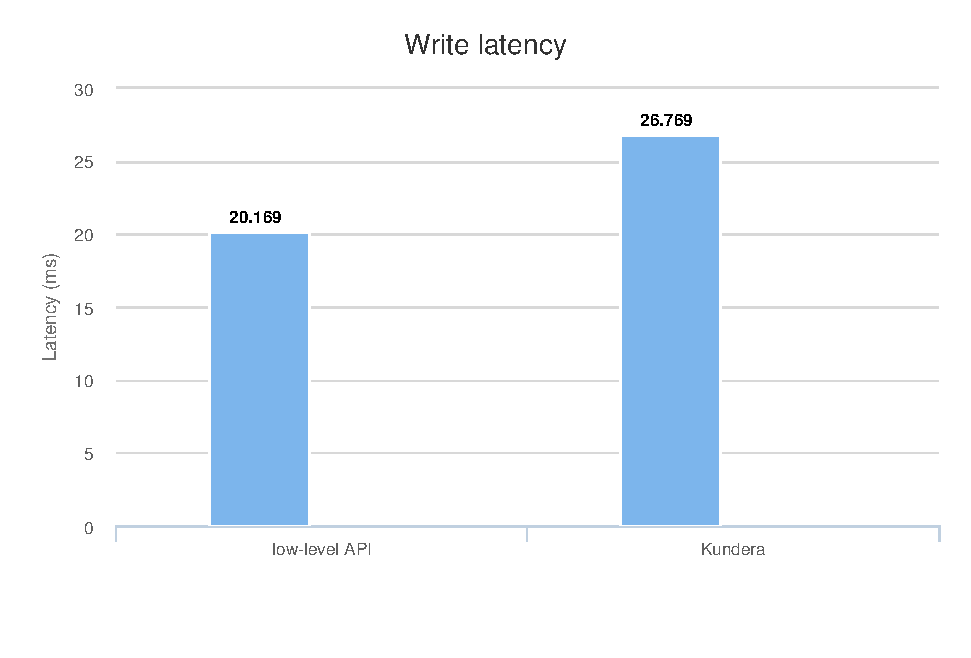
\includegraphics[width=7cm]{images/hbase_write_latency}
  }
  \caption{HBase - write operation benchmark results}
  \label{fig:hbase-test-write}
\end{figure} 

\noindent Even if the tests for HBase has been made on a local instance of the database, they show a similar behavior with respect to the tests executed over the network for Google Datastore and Azure Tables.

\subsection{Discussion}
\label{sec:discussion}
The main objective of our tests was to guarantee that the loss of performance, between the Kundera version of the client and the client written with direct use of the low-level API, was minimum or at least not as much to discourage the use of the JPA approach for NoSQL databases.

\noindent Since Kundera provides a set of benchmark results obtained through YCSB, and since they show an acceptable performance loss, our objective included the comparison of our results with the results obtained by Kundera. Kundera executes its tests on instances of the databases that reside on a local testing machine, since it is meaningless for us to test the developed extensions against their local emulator due to the fact that Google Datastore and Azure Tables are NoSQL databases developed for DaaS, we cannot directly compare our results with the Kundera ones.

\noindent The idea was to replicate the results of Kundera on HBase, executing the tests, no more on a local instance of HBase but on a remote instance that was deployed in the Politecnico di Milano cloud. Unfortunately the comparison of the results cannot be done due to malfunctioning of the HBase cluster on the Politecnico di Milano cloud.

\newparagraph As can be seen from comparing the values of the throughput of HBase and those of the tests on Google Datastore and Azure Tables, while tests are executed over the network, throughput drops significantly.
YCSB tries to go as fast as possible in issuing operation on the database instance trying to reach the maximum throughput the system can afford. The cause of the throughput drop is due to the high number of TCP connections that need to be maintained during the benchmark execution; in fact, each requests needs a TCP connection to be opened and maintained, at least until the response comes from the server. When executing the tests with 100.000 entities this becomes the bottleneck for the benchmark.

\noindent Similar considerations hold for the latency, the values reported for Google Datastore and Azure Tables, include the round trip time of the requests and furthermore it depends on the state of network congestion. By looking at the network consumption data reported by the operating system of the testing machine, we estimated that the average round trip time, during the tests, was of 56,29 ms.

\newparagraph After these considerations, and by looking at the differences in both throughput and latency for the low-level API and the developed Kundera extension, we conclude that a performance loss exists, but is not enough to discourage the usage of those NoSQL databases through Kundera, especially given the benefits this solution brings in working with NoSQL databases.

\section{Summary}
In this chapter we have presented the test driven approach used to develop the Kundera extensions. Then we described how we prepared and executed the test of correctness and performance made for the two developed Kundera extension, showing the minimal performance loss that Kundera add to the low-level API.
Finally we have presented \textit{Hegira-generator}, the application developed to test the mechanisms encapsulated inside CPIM to interacts with the synchronization system.
